\documentclass[svgnames,11pt]{beamer}
\input{/home/tof/Documents/Cozy/latex-include/preambule_commun.tex}
\input{/home/tof/Documents/Cozy/latex-include/preambule_beamer.tex}
\usepackage{pgfpages} \setbeameroption{show notes on second screen=left}
\author[]{Christophe Viroulaud}
\title{Première page web}
\date{\framebox{\textbf{Web 01}}}
%\logo{}
\institute{Seconde - SNT}

\begin{document}
\begin{frame}
    \titlepage
        \note{\fcolorbox{black}{red}{{\LARGE mettre sur site à partir 3}}}
\end{frame}
\begin{frame}
    \frametitle{}

    \begin{center}
        Le \emph{Web} a révolutionné la manière de communiquer des humains. Il permet de présenter des contenus de manière illimitée et à n'importe quelle personne connectée.
    \end{center}

\end{frame}
\begin{frame}
    \frametitle{}

    \begin{framed}
        \centering Comment construire un contenu visualisable sur le Web?
    \end{framed}

\end{frame}
\section{Histoire du Web}
\begin{frame}
    \frametitle{Histoire du web}

    \begin{center}
        \centering
        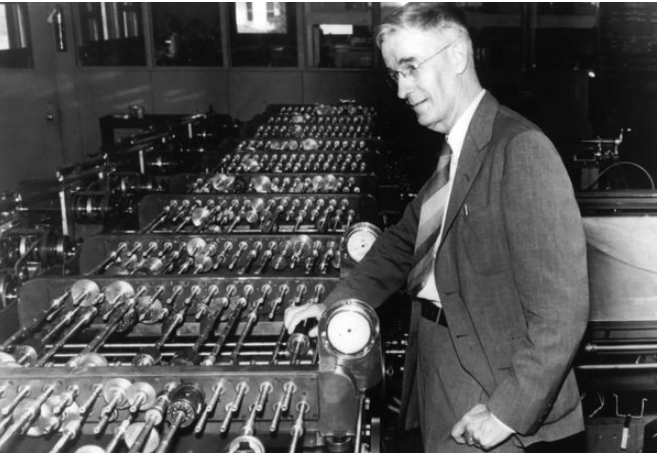
\includegraphics[width=6cm]{ressources/bush.png}
        \captionof{figure}{1945: Vannevar Bush}
        \label{IMG}
    \end{center}
    \begin{aretenir}[]
        Il publie un article "\emph{as we may think}" où il prédit l'invention de l'hypertexte. Il décrit un système (le Memex) qui permet "d'étendre la mémoire de l'Homme"
    \end{aretenir}
\end{frame}
\begin{frame}
    \frametitle{}

    \begin{center}
        \centering
        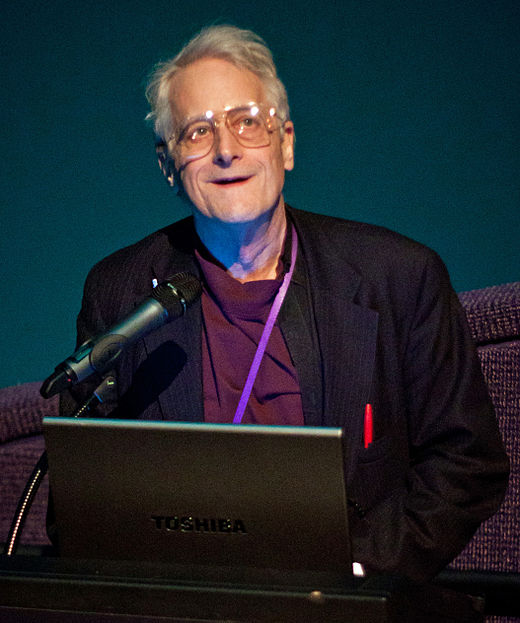
\includegraphics[width=4cm]{ressources/nelson.jpg}
        \captionof{figure}{1965: Ted Nelson}
        \label{IMG}
    \end{center}
    \begin{aretenir}[]
        Il développe la notion d'\textbf{hypertexte}: un ensemble de documents reliés entre eux par des hyperliens.
    \end{aretenir}
\end{frame}
\begin{frame}
    \frametitle{}

    \begin{center}
        \centering
        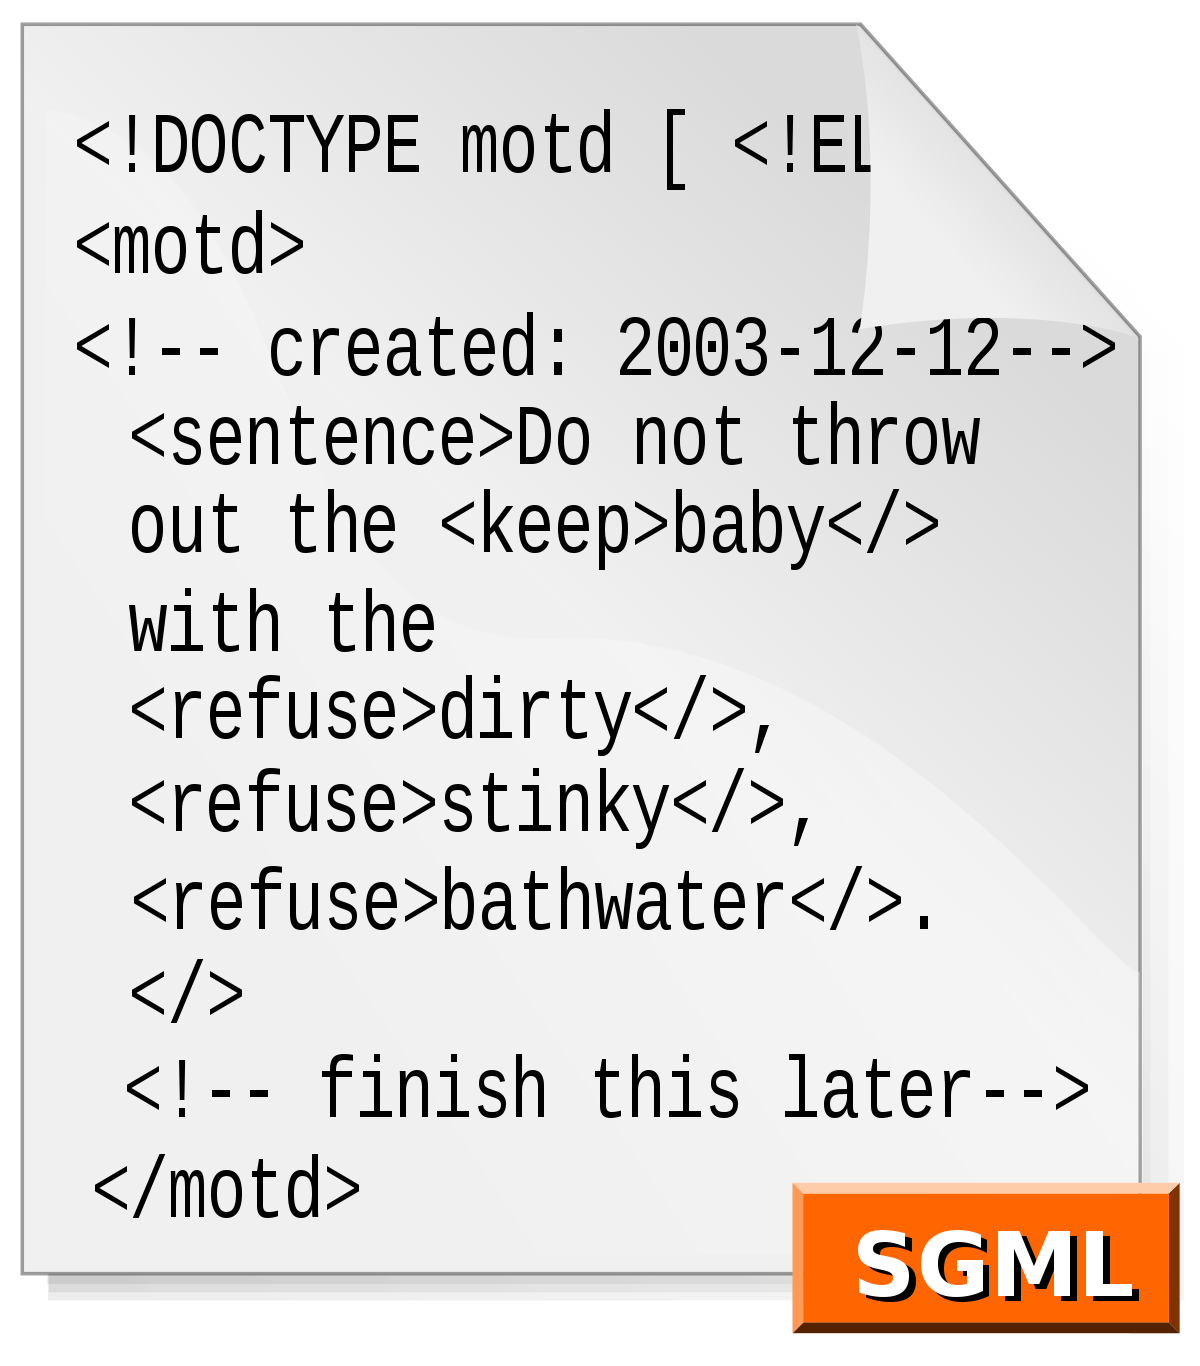
\includegraphics[width=4cm]{ressources/sgml.png}
        \captionof{figure}{1980 - 1984: SGML}
        \label{IMG}
    \end{center}
    \begin{aretenir}[]
        \textbf{Standard Markup General Language:} Langage basé sur le concept de balises et de liens hypertextes. Adopté par de nombreuses institutions et entreprises (comme le CERN).
    \end{aretenir}
\end{frame}
\begin{frame}
    \frametitle{}

    \begin{center}
        \centering
        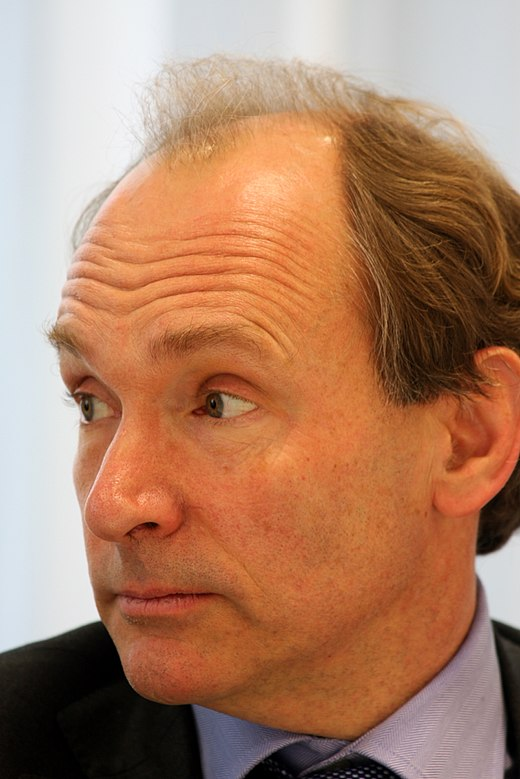
\includegraphics[width=3.5cm]{ressources/lee.jpg}
        \captionof{figure}{1989: Tim Berners-Lee}
        \label{IMG}
    \end{center}
    \begin{aretenir}[]
        Il est considéré comme le père du web. Il travaille au CERN (Organisation Européenne pour la Recherche Nucléaire)
    \end{aretenir}
\end{frame}
\begin{frame}
    \frametitle{}

    Tim Berners-Ler développe les 3 principales technologies du web:
    \begin{itemize}
        \item<1-> \textbf{URL (Uniform Resource Locator): }adresse d'une ressource donnée, unique sur le Web.
        \item<2-> \textbf{HTTP (HyperText Transfer Protocol): }protocole de communication client-serveur.
        \item<3-> \textbf{HTML (HyperText Markup Language): } (version simplifiée du SGML) langage conçu pour représenter les pages web.
    \end{itemize}

\end{frame}
\begin{frame}
    \frametitle{}

    \begin{center}
        \centering
        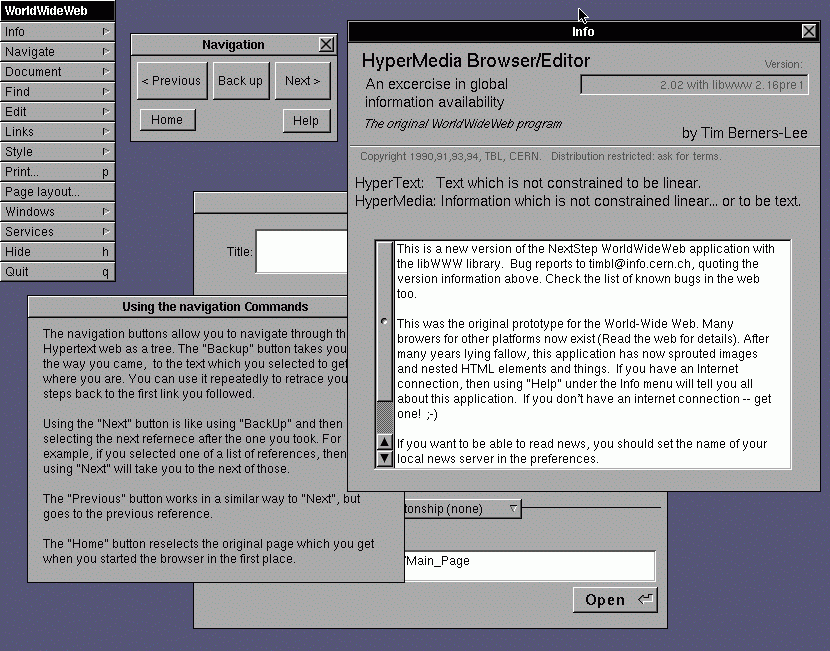
\includegraphics[width=6cm]{ressources/WorldWideWeb.png}
        \captionof{figure}{1990: Premier navigateur \emph{WorldWideWeb}}
        \label{IMG}
    \end{center}
    \begin{aretenir}[]
        Tim Berners-Lee développe le premier navigateur. Le Web est d'abord utilisé par les physiciens pour partager leurs recherches.
    \end{aretenir}
    \note{www: grande toile mondiale}
\end{frame}
\begin{frame}
    \frametitle{}

    \begin{center}
        \centering
        
\includegraphics[width=4cm]{ressources/milliard.png}
        \captionof{figure}{2014: un milliard de sites web}
        \label{IMG}
    \end{center}
    \begin{aretenir}[]
        Le 30 avril 1993, le CERN décide de déposer les technologies du Web dans le \textbf{domaine public}.
    \end{aretenir}
    \note{8 mars 2021: 1,84 milliards; seulement 200 millions vraiment actifs}
\end{frame}
\section{Un langage: HTML}
\subsection{Langage de balises}
\begin{frame}[fragile]
    \frametitle{HTML: un langage de balises}

    Le \emph{HTML} un langage de balises c’est à dire que chaque composant de la page (texte, image, lien hypertexte...) est inséré grâce à des blocs spécifiques.
    \begin{center}
        \begin{lstlisting}[language=html , basicstyle=\ttfamily\small, xleftmargin=2em, xrightmargin=2em]
<html>

</html>
\end{lstlisting}
        \captionof{code}{Bloc principal}
        \label{CODE}
    \end{center}
\end{frame}
\subsection{Squelette principal}
\begin{frame}[fragile]
    \frametitle{Squelette principal}

    La plupart des blocs sont définis avec une balise ouvrante (exemple : \texttt{\textbf{<html>}}) et une balise fermante (exemple : \texttt{\textbf{</html>}}).
    \begin{center}
        \begin{lstlisting}[language=html , basicstyle=\ttfamily\small, xleftmargin=2em, xrightmargin=2em]
<html>
    <head>

    </head>
    <body>

    </body>
</html>
\end{lstlisting}
        \captionof{code}{Squelette principal}
        \label{CODE}
    \end{center}
\end{frame}
\begin{frame}[fragile]
    \frametitle{}
    \begin{lstlisting}[language=html , basicstyle=\ttfamily\small, xleftmargin=2em, xrightmargin=2em]
<html>
    <head>

    </head>
    <body>

    </body>
</html>
\end{lstlisting}
    \begin{activite}
        \begin{enumerate}
            \item Créer un dossier \textbf{\texttt{premiere-page}}
            \item Ouvrir le bloc-notes \emph{Windows}.
            \item Dans le dossier, enregistrer le fichier sous le nom \textbf{\texttt{page-votrenom.html}} . \underline{Attention:} le nom ne devra contenir aucun espace ni accent.
            \item Recopier le squelette de la page web.
        \end{enumerate}
    \end{activite}

\end{frame}
\subsection{head}
\begin{frame}[fragile]
    \frametitle{head}

    Le bloc \textbf{\texttt{head}} permet d'interagir avec le navigateur.
    \begin{activite}
        Ajouter le bloc \textbf{\texttt{title}} dans le bloc \textbf{\texttt{head}}. Il permet de créer le titre qui s'affiche dans la barre du navigateur.
        \begin{center}
            
\includegraphics[width=8cm]{ressources/head.png}

        \end{center}
        \begin{lstlisting}[language=html , basicstyle=\ttfamily\small, xleftmargin=2em, xrightmargin=2em]
<head>
    <title>Le titre de ma page</title>
</head>
\end{lstlisting}
    \end{activite}

\end{frame}
\subsection{body}
\begin{frame}[fragile]
    \frametitle{body}

    Le bloc \textbf{\texttt{body}} regroupe tout le contenu de la page.
    \begin{activite}
        Ajouter le bloc \textbf{\texttt{p}} (pour paragraphe) dans le bloc \textbf{\texttt{body}}.
        \begin{lstlisting}[language=html , basicstyle=\ttfamily\small, xleftmargin=2em, xrightmargin=2em]
<body>
    <p>Mon premier contenu</p>
</body>
\end{lstlisting}
    \end{activite}

\end{frame}
\subsection{Visualiser la page}
\begin{frame}
    \frametitle{Visualiser la page}

    Une page \textbf{\texttt{html}} se lit avec un navigateur.

    \begin{activite}
        \begin{enumerate}
            \item Ouvrir \emph{Firefox} ou \emph{Chrome}.
            \item Ouvrir la page web avec le navigateur.
            \item Remarquer le titre de la page, le contenu affiché dans le navigateur.
        \end{enumerate}
    \end{activite}
\end{frame}
\subsection{Ajouter du contenu}
\subsubsection{Blocs principaux}
\begin{frame}
    \frametitle{Ajouter du contenu - blocs principaux}
    Pour construire une page plus riche, il faut connaître quelques blocs:
    \begin{itemize}
        \item paragraphe,
        \item titre,
        \item liste,
        \item image,
        \item lien hypertexte.
    \end{itemize}


\end{frame}
\subsubsection{Paragraphe}
\begin{frame}[fragile]
    \frametitle{Paragraphe}
    Chaque nouveau paragraphe doit être insérer dans une balise \textbf{\texttt{p}}.

    \begin{center}
        \begin{lstlisting}[language=html , basicstyle=\ttfamily\small, xleftmargin=2em, xrightmargin=2em]
<p>Blablabla</p>

<p>Blablablablablabla</p>
\end{lstlisting}
    \end{center}
    \begin{center}
        \centering
        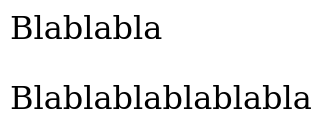
\includegraphics[width=8cm]{ressources/paragraphe.png}
        \captionof{figure}{Rendu}
        \label{IMG}
    \end{center}
\end{frame}
\subsubsection{Titre}
\begin{frame}[fragile]
    \frametitle{Titre}
    Il est possible de créer six niveaux de titre avec les balises \textbf{\texttt{h1}} à \textbf{\texttt{h6}}.
    \begin{center}
        \begin{lstlisting}[language=html , basicstyle=\ttfamily\small, xleftmargin=2em, xrightmargin=2em]
<h1>Un titre</h1>
<h2>Un sous-titre</h2>
<h3>Un sous-sous-titre</h3>
\end{lstlisting}
    \end{center}
    \begin{center}
        \centering
        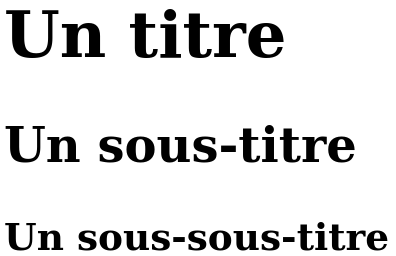
\includegraphics[width=7cm]{ressources/titre.png}
    \end{center}
\end{frame}
\subsubsection{Liste}
\begin{frame}[fragile]
    \frametitle{Liste}
    On crée une liste avec le bloc \textbf{\texttt{ul}}. Chaque item est ajouté avec le bloc \textbf{\texttt{li}}.
    \begin{center}
        \begin{lstlisting}[language=html , basicstyle=\ttfamily\small, xleftmargin=2em, xrightmargin=2em]
<ul>
    <li>premier point</li>
    <li>deuxième point</li>
    <li>troisième point</li>
</ul>
\end{lstlisting}
    \end{center}
    \begin{center}
        \centering
        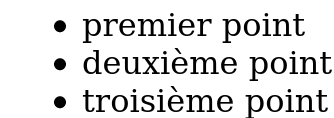
\includegraphics[width=7cm]{ressources/liste.png}
    \end{center}
\end{frame}
\subsubsection{Image}
\begin{frame}
    \frametitle{Image}
    Pour illustrer la page on peut ajouter une image avec la balise \textbf{\texttt{img}}.

    Il faut d'abord posséder une image \textbf{dans le même dossier} que la page web. Le nom de l'image ne doit pas contenir d'espace ni d'accent.
    \begin{center}
        \centering
        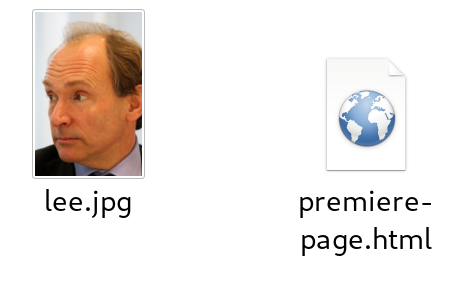
\includegraphics[width=8cm]{ressources/dossier-img.png}
        \captionof{figure}{L'image est dans le même dossier que la page.}
        \label{IMG}
    \end{center}
\end{frame}
\begin{frame}[fragile]
    \frametitle{}

    La balise ouvrante \textbf{\texttt{img}} n'a pas de balise fermante. Elle possède des \textbf{attributs}:
    \begin{itemize}
        \item \textbf{\texttt{src:}} \emph{(obligatoire)} adresse de l'image,
        \item \textbf{\texttt{alt:}} \emph{(facultatif)} texte alternatif.
    \end{itemize}
    \begin{center}
        \begin{lstlisting}[language=html , basicstyle=\ttfamily\small, xleftmargin=0.5em, xrightmargin=-1em]
<img src="lee.jpg" alt="Portrait de Tim Berners-Lee">
\end{lstlisting}
    \end{center}


\end{frame}
\subsubsection{Lien hypertexte}
\begin{frame}[fragile]
    \frametitle{Lien hypertexte}

    Une page web sans lien vers d'autres pages n'a pas grand intérêt. La balise \textbf{\texttt{a}} est une des plus importantes du langage \textbf{\texttt{html}}.\\L'attribut \textbf{\texttt{href}} contient l'adresse de la page à visiter.
    \begin{center}
        \begin{lstlisting}[language=html , basicstyle=\ttfamily\small, xleftmargin=0.1em, xrightmargin=-1.8em]
<a href="https://lyceejaydebeaufort.fr/">Page de Jay</a>
\end{lstlisting}
        \captionof{code}{Lien vers une page externe.}
    \end{center}

    \begin{center}
        \centering
        
\includegraphics[width=5cm]{ressources/lien.png}
    \end{center}

\end{frame}
\section{Page web sur l'orientation}
\begin{frame}
    \frametitle{Page web sur l'orientation}

    \begin{activite}
    Compléter la page web pour présenter le projet d'orientation. La page sera décomposée en trois parties:
    \begin{itemize}
        \item métier(s) envisagé(s) (ou catégorie)
        \item études post-bac à réaliser
        \item spécialités (ou filière technologique) à choisir
    \end{itemize}
    Il faudra utiliser les balises présentées pour mettre en forme le contenu. La page devra contenir au moins une image d'illustration ainsi qu'un lien externe.
    \end{activite}

\end{frame}
\end{document}